\section{阶跃函数和冲激函数}
函数本身有不连续点(跳变点)或其导数与积分有不连续点的一类函数统称为奇异信号或奇异函数。
\subsection{单位阶跃函数}

\begin{Figure}[单位阶跃函数]
    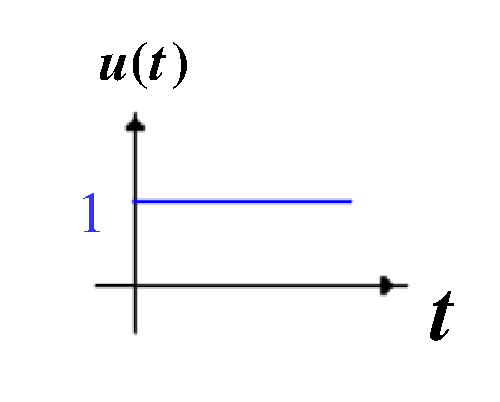
\includegraphics[width=40mm]{visio/1.12.pdf}
\end{Figure}

\begin{BoxDefinition}[单位阶跃函数]
    单位阶跃函数
    \begin{Equation}
        u(t)=\left\{
        \begin{aligned}
            1 & , & t > 0 \\
            0 & , & t < 0
        \end{aligned}
        \right.
    \end{Equation}
    $t=0$处发生跳变,或认为$u(t)=\frac{1}{2}$
\end{BoxDefinition}

对单位阶跃函数作平移可得延迟单位阶跃信号。

\begin{BoxProperty}[单位阶跃函数的性质]
    可以通过平移和加减运算表示某些函数

    可以表示某些函数的区间(乘上阶跃函数的组合)

    阶跃函数的积分

    \begin{Equation}
        \int_{-\infty}^{t} \varepsilon(\tau) d\tau = t\varepsilon(t)
    \end{Equation}
\end{BoxProperty}

\subsection{单位冲激函数}

\begin{Figure}[单位冲激函数]
    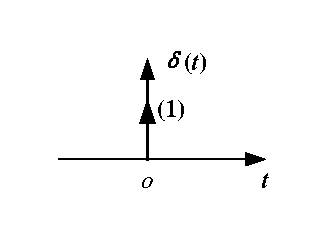
\includegraphics[width=40mm]{visio/1.13.pdf}
\end{Figure}

\begin{BoxDefinition}[单位冲激函数]
    设一矩形脉冲$p_{\tau}(t)$的宽为$\tau$,高为$\frac{1}{\tau}$,面积为$1$
    \begin{Equation}
        \delta(t) = \lim\limits_{\tau\rightarrow 0} p_{\tau}(t)
    \end{Equation}
    或由狄拉克定义
    \begin{Equation}
        \left\{
        \begin{array}{ll}
            \delta (t) = 0 & (t \neq 0) \\
            \int_{-\infty}^{\infty} \delta (t)dt=1
        \end{array}
        \right.
    \end{Equation}
    且
    \begin{Equation}
        \int_{-\infty}^{\infty} \delta (t)dt= \int_{0_{-}}^{0_{+}} \delta (t)dt = 1
    \end{Equation}
    $t=0$时,$\delta(t)\rightarrow \infty$,为无界函数。
\end{BoxDefinition}

\subsection{冲激函数的性质}

\begin{BoxProperty}[冲激函数的取样性]*
    冲激函数的取样性
    \begin{Equation}
        f(t)\delta(t)=f(0)\delta(t) \\
    \end{Equation}
    \begin{Equation}
        \int_{-\infty}^{\infty} f(t)\delta(t)dt = f(0)
    \end{Equation}
\end{BoxProperty}

\begin{BoxProperty}[冲激函数的奇偶性]
    冲激函数为偶函数
    \begin{Equation}
        \delta(-t)=\delta(t)
    \end{Equation}
\end{BoxProperty}

\begin{BoxProperty}[冲激函数的比例性]
    冲激函数的展缩变换有以下性质
    \begin{Equation}
        \delta(at)=\frac{1}{|a|}\delta(t)
    \end{Equation}
    结合平移
    \begin{Equation}
        \delta(at-t_0)=\frac{1}{|a|}\delta(t-\frac{t_0}{a})
    \end{Equation}
\end{BoxProperty}

\begin{BoxProperty}[冲激函数的微积分性质]
    冲激函数与阶跃函数有以下关系
    \begin{Equation}
        \varepsilon (t) = \int_{-\infty}^{t} \delta (\tau) d\tau
    \end{Equation}
    或
    \begin{Equation}
        \delta (t) = \frac{d\varepsilon(t)}{dt}
    \end{Equation}
\end{BoxProperty}

引入冲激函数后,间断点导数也连续。

\begin{BoxProperty}[复合函数形式的冲激函数]
    设$f(t)$有$n$个不相等的实根$t_i(i=1,2,\dots,n)$,则
    \begin{Equation}
        \delta[f(t)]=\sum\limits_{i=1}^n\frac{1}{|f'(t_i)|}\delta(t-t_i)
    \end{Equation}
    若$f(t)$有重根,则$\delta[f(t)]$无意义。
\end{BoxProperty}

\begin{Figure}[冲激偶]
    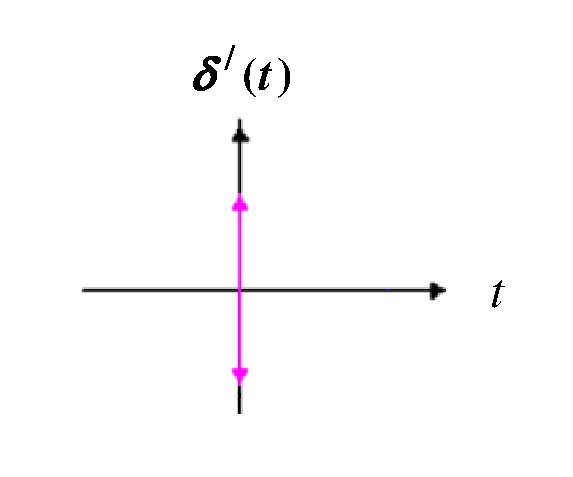
\includegraphics[width=60mm]{visio/add1.pdf}
\end{Figure}

\begin{BoxProperty}[冲激偶的性质]
    冲激偶即冲激函数的导数,有以下性质
    \begin{Equation}
        f(t)\delta'(t)=f(0)\delta'(t)-f'(0)\delta(t)
    \end{Equation}
    \begin{Equation}
        \int_{-\infty}^{\infty} f(t)\delta'(t)dt = -f'(0)
    \end{Equation}
    \begin{Equation}
        \int_{-\infty}^{t} \delta'(t)dt = \delta(t)
    \end{Equation}
    \begin{Equation}
        \int_{-\infty}^{\infty} \delta'(t)dt = 0
    \end{Equation}
    \begin{Equation}
        \delta^{(n)}(at)=\frac{1}{|a|}\cdot\frac{1}{a^n}\delta^{(n)}(t)
    \end{Equation}
\end{BoxProperty}

\subsection{单位样值序列和单位阶跃序列}

\subsubsection{单位样值序列}

\begin{Figure}[单位样值序列]
    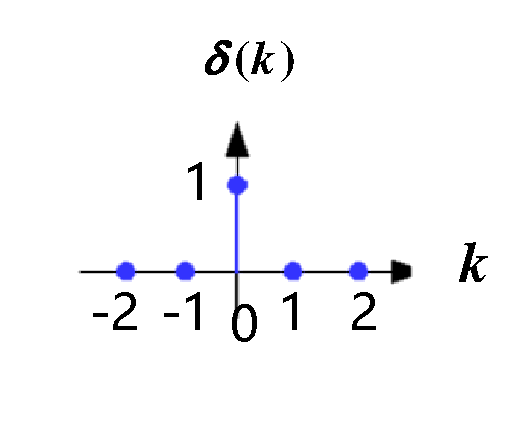
\includegraphics[width=40mm]{visio/1.14.pdf}
\end{Figure}

\begin{BoxDefinition}[单位样值序列]
    单位样值序列
    \begin{Equation}
        \varepsilon (k) \overset{\mathrm{def}}{=}
        \left\{
        \begin{aligned}
            1 & , & k = 0    \\
            0 & , & k \neq 0
        \end{aligned}
        \right.
    \end{Equation}
\end{BoxDefinition}


\begin{BoxProperty}[单位样值序列的取样性]
    单位样值序列的取样性
    \begin{Equation}
        f(k)\delta(k-k_0)=f(k_0)\delta(k-k_0)
    \end{Equation}
    \begin{Equation}
        \sum_{k=-\infty}^{\infty}f(k)\delta(k-k_0) = f(k_0)
    \end{Equation}
\end{BoxProperty}

\subsubsection{单位阶跃序列}

\begin{Figure}[单位阶跃序列]
    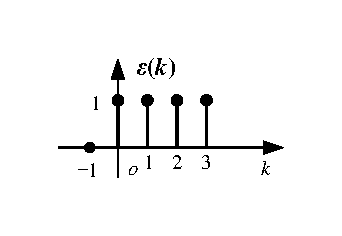
\includegraphics[width=60mm]{visio/1.15.pdf}
\end{Figure}

\begin{BoxDefinition}[单位阶跃序列]
    单位阶跃序列
    \begin{Equation}
        \varepsilon (k) \overset{\mathrm{def}}{=}
        \left\{
        \begin{aligned}
            1 & , & k \geq 0    \\
            0 & , & k < 0
        \end{aligned}
        \right.
    \end{Equation}
\end{BoxDefinition}

\begin{BoxProperty}[单位样值序列和单位阶跃序列的关系]
    单位样值序列和单位阶跃序列的关系
    \begin{Equation}
        \delta (k) = \varepsilon(k) - \varepsilon(k-1)
    \end{Equation}
    \begin{Equation}
        \varepsilon(k) = \delta(k) + \delta(k-1) + \dots
    \end{Equation}
\end{BoxProperty}


